\begin{figure}[H]
    \centering
    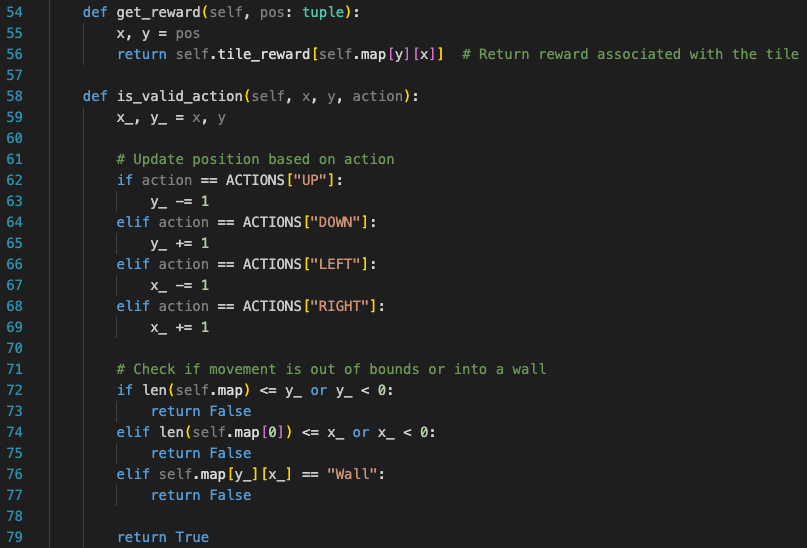
\includegraphics[width=0.8\textwidth]{images/helper_func.png}
    \caption{Helper Methods}
    \label{fig:helper}
\end{figure}

Figure~\ref{fig:helper} illustrates the \texttt{get\_reward} and \texttt{is\_valid\_action} methods, which are integral to both algorithms. The \texttt{get\_reward} method retrieves the corresponding reward or penalty for a given state, ensuring that the agent correctly perceives its environment. Meanwhile, the \texttt{is\_valid\_action} method verifies the feasibility of an action by preventing the agent from moving into a Wall cell, thereby enforcing state constraints and ensuring that invalid moves result in the agent remaining in its current position.
